
%%%%%%%%%%%%%%%%%%%%%%%%%%%%%%% INTRO %%%%%%%%%%%%%%%%%%%%%%%%%%%%%

%We attach unique identifiers to type holes, interpret them as type variables, and infer types for holes with Hindley-Milner \emph{type inference} \cite{MilnerInfer} based on unification \cite{RobinUnification}. The algorithm follows two standard steps, constraint generation and constraint solving by unification.

%The implementation inserts holes automatically, following the \Hazelnut edit action calculus, to guarantee that every editor state has some (possibly incomplete) type.

\section{Type Hole Inference Introduction}
\label{sec:intro}
\emph{Bidirectional typing} and \emph{constraint-based type inference} are common approaches to deducing types for partially annotated programs. \emph{Bidirectional typing} is a simple algorithmic system with type information propagating from the outside in \cite{BidirTyping}. This produces clear error messages at the cost of requiring explicit type annotations in certain situations, e.g. top-level functions. \emph{Type inference} allows programmers to omit most or all type annotations, but requires complex constraint solving for type checking, making it difficult for users to reason about types and producing complex error messages \cite{typeinferDif}.
This paper develops \emph{type hole inference}, which combines the benefits of bidirectional typing and type inference.\par

In recent work on the \Hazel programming environment, \citet{HazelnutPOPL} assign formal meaning to incomplete programs, i.e. programs with holes, by developing a bidirectional type system with support for expression and type holes. Type holes operate as the unknown types from gradual type theory \cite{GradualTyping}. Our approach takes this type system and adds constraint solving as a layer on top to suggest type hole fillings, without making constraint solving necessary for typing. Take the following \Hazel programs extended with type hole inference as examples: 
\begin{figure}[htbp]
\centering
  \begin{tabular}[b]{cc}
    \begin{tabular}[b]{c}
      \begin{subfigure}[b]{0.4\columnwidth}
        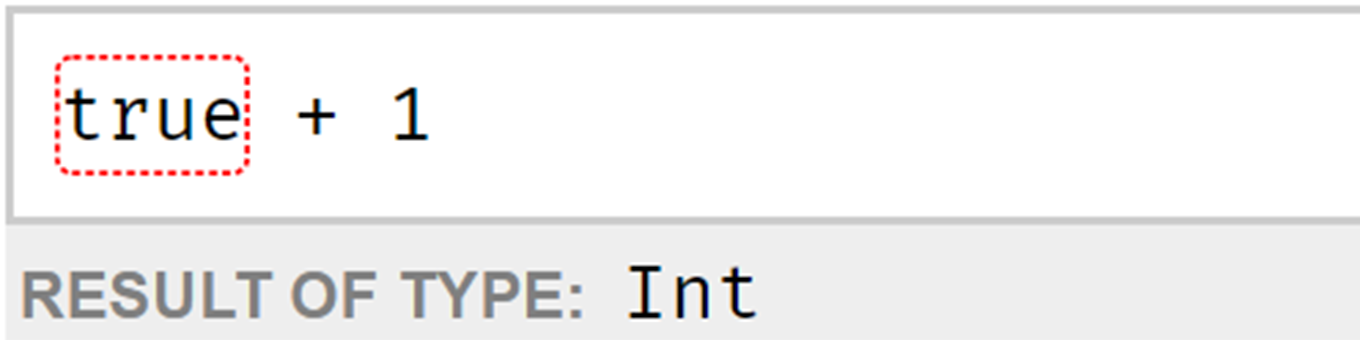
\includegraphics[width=5.5cm]{images/3_1.png}
        \caption{Example of static error}
        \label{fig:staticerror}
      \end{subfigure}\\
      \begin{subfigure}[b]{0.4\columnwidth}
        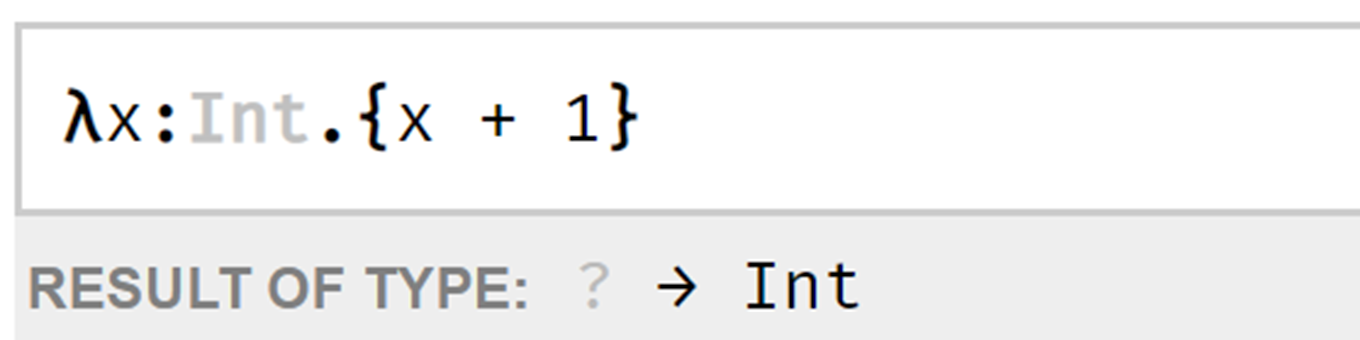
\includegraphics[width=5.5cm]{images/4_gray.png}
        \caption{Example of constraint solving success}
		\label{fig:unifsuc}
      \end{subfigure}
    \end{tabular}
    &
     \begin{tabular}[b]{c}
          \begin{subfigure}[b]{0.4\columnwidth}
      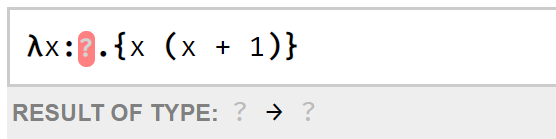
\includegraphics[width=5.5cm]{images/unifyfail_2.png}
      \caption{Example of constraint solving failure}
	\label{fig:uniffail}
	\end{subfigure}\\
      \begin{subfigure}[b]{0.4\columnwidth}
        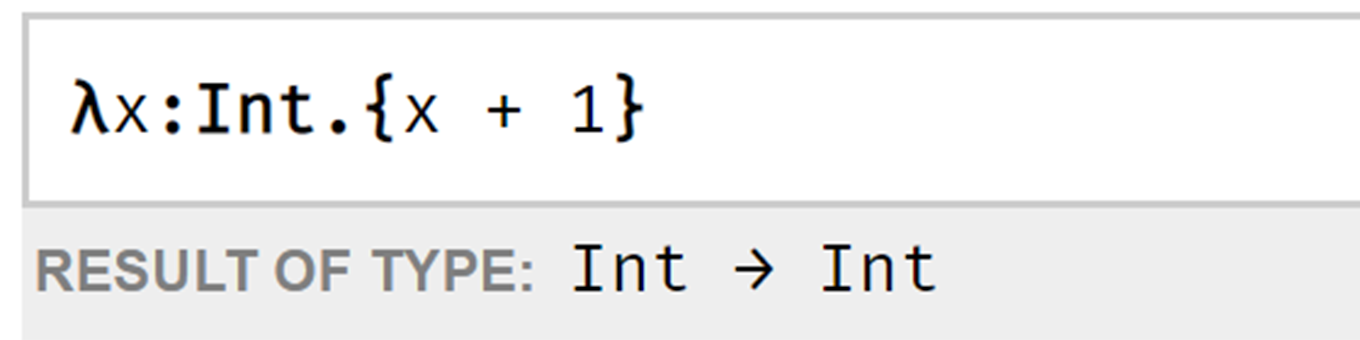
\includegraphics[width=5.5cm]{images/4_black.png}
        \caption{Example of filling type holes}
		\label{fig:fillholeeg}
      \end{subfigure}
    \end{tabular}
  \end{tabular}
  \caption{Programs in Hazel environment}
  \vspace{-2px}
\end{figure}
\par Figure ~\ref{fig:staticerror} fails type checking at bidirectional typing, so our system reports a static error. Bidirectional judgements easily trace back the error and indicate the source in the editor with a red box, showing that the operand should be $Int$ type. \par 
Figure ~\ref{fig:unifsuc} is an example succeeding in both static checking and constraint solving.  The bidirectional typing requires that a type annotation be provided on the lambda, but it is left as a hole. The system synthesizes the "$\tarr{?}{Int}$" type, with "$?$" standing for hole type. The constraint solver then generates a solution, $[(?,~ Int)]$, for the hole. Hence, the type hole is filled with a gray "$Int$" in the editor. The programmer can use a keyboard shortcut to replace the type hole with the suggested type as shown in Figure ~\ref{fig:fillholeeg}, and the expression is synthesized to "$\tarr{Int}{Int}$" after replacement. \par

Figure ~\ref{fig:uniffail} is an example failing in constraint solving. Constraints, $(? \approx Int)$ and $(? ~ \approx ~ \tarr{?}{?})$, conflict since the type hole can not be $Int$ and $arrow \, type$ at the same time. In this case, the expression still remains well-typed since $x$ is of hole type. The system postpones type-checking to runtime. However, the failure to infer a type is visually reported to indicate the issue.

\emph{Type hole inference} has a simple typing algorithm, simple error messages, and explicit annotations in the same situations that bidirectional typing does. However, programmers don't have to actually fill out those explicit annotations, most of which are type holes inserted and filled by the \emph{type hole inference} automatically as shown in Figure ~\ref{fig:unifsuc}. The algorithm treats type holes as unknown types, and regards expressions well-typed no matter how constraint solving goes. 
%Besides, types that are generated by constraint solving always relate to a syntactic type hole in the code, so there is always somewhere to display them in the editor.
% The problem is that limited type information for type holes gained through bidirectional typing judgements \cite{HazelLive}. \par

% \citet{HazelnutPOPL} derived \emph{type holes} coinciding with machinery of gradual typing \cite{GraualTyp}, identifying type holes as unknown types. We 

% Inferring types for type holes turns to be a problem of realizing type inference on gradual typing system. 

%  To combine type inference with gradual typing, \citet{GradualInfer} came up an inference algorithm with design space under conditions that three straightforward approaches fail. One simple approach that replaces unknown types with a fresh variable and apply type inference does not work because unexpected static error is triggered when an unknown type is equal to multiple types \cite{GradualInfer}. However, starting from static semantics extended with \emph{holes} gives a new insight to this approach. The type holes corresponding to the unknown type can be filled with hole type to keep programs well-typed when unification fails, and delay type checking for those holes to runtime rather than raise a static error. Our approach is easy to implement by introducing holes into the type inference algorithm \cite{TaplBook}.

% We extended static semantics with \emph{type constraints}, and borrow machinery from unification-based type inference to infer types for type holes by identifying the type hole with the type variable. In particular, our system will not report a static error when unification fails but postpone type-checking for type holes to runtime. This provides an approach to combine \emph{gradual typing} and \emph{type inference}. 
\par{Contributions} The contributions of this paper are: (1) a new bidirectional typing system extended with type constraints in section ~\ref{sec:typinf}; (2) a type inference algorithm to handle type holes in section ~\ref{sec:infalg}.

%Programmers have to deal with incomplete programs like syntactically malformed edit states during development.

%%%%%%%%%%%%%%%%%%%%%%%%%%%%%%% TYPE SYSTEM %%%%%%%%%%%%%%%%%%%%%%%%%%%%%

\section{Type System for Type Hole Inference}

\label{sec:typinf}
Figure ~\ref{fig:syntax_fig} defines the syntax of H-types and H-expressions. We start from the definition given in \citet{HazelnutPOPL} except two modifications. First, we add an annotated lambda. Second, we attach a unique \emph{type hole identifier}, drawn as a superscript capital letter, to each type hole, such as $\ehole^A$. In this way, type holes are identified as type variables. There are two types of expression holes: empty holes, $\ehole$, standing for missing parts of an incomplete program, and non-empty holes, $\notehole{e}$, operating as membranes around static and dynamic type inconsistencies \cite{HazelLive}. \par
\begin{figure}[htbp]
\vspace{-3px} 
$\arraycolsep=4pt\begin{array}{lll}
HProv~~ p & ::= & 
    n ~\vert~ 
    \rightarrow_{L}(p) ~\vert~ 
    \rightarrow_{R}(p)
    \\
HTyp~~ \tau & ::= &
  \tnum ~\vert~
  \tbool ~\vert~
  \tarr{\tau}{\tau} ~\vert~
  \ehole^p
  \\
HExp~~ e & ::= &
  x ~\vert~
  \lamfunc{x}{e} ~\vert~
  \lamfunc{x:\tau}{e} ~\vert~
  e(e) ~\vert~
  \underlinenum{n} ~\vert~
  (e+e) ~\vert~
  e: \tau ~\vert~
  \ehole  ~\vert~
  \notehole{e} 
\end{array}$
\hrule
\caption{Syntax of H-types, H-expressions, and Type Constraint Set}
\label{fig:syntax_fig}
\vspace{-5px}
\end{figure}
Figure ~\ref{fig:ana-syn} defines a bidirectional typing system extended with type constraint sets. \emph{Type constraint set} $C$ is a set of type consistency relations, namely \emph{type constraints}. We use a union operation, $C \cup C$, corresponding to mathematical set union operation to generate constraints inductively through bidirectional propagation. The type constraint set is solved by the unification algorithm in section ~\ref{sec:infalg}, but importantly, constraint solving is not necessary for typing to succeed. The typing context, $\Gamma$, maps a set of expression variables to their types. Rule ~\ref{rule:syn-ehole} and ~\ref{rule:syn-hole} synthesize expression hole to hole type, with premise, $(n ~ \text{fresh})$, indicating generation of a new \emph{type identifier}. Rule ~\ref{rule:ana-subsume} and ~\ref{rule:ana-lam} have type consistency in their premises, generating new constraints and merging them into constraint sets in the conclusion. Rule ~\ref{rule:syn-ap}, ~\ref{rule:ana-lam} and ~\ref{rule:ana-lamann} have \emph{matched arrow type judgements} defined in figure ~\ref{fig:match-arrow-typ}. They leave the arrow type unchanged and assign the type hole the matched arrow type $\tarr{\tehole^{\rightarrow_{L}(p)}}{\tehole^{\rightarrow_{R}(p)}}$ where new holes are uniquely identified by matched arrow provenances generated from the original hole $\tehole^{p}$ and constraint generation links the original hole to its matched counterpart \cite{HazelnutPOPL}.
\begin{figure}[htbp]
\vspace{-3px} 
    \begin{multicols}{2}
      \fbox{$\consexptyp{\Gamma}{e}{\tau}{C}$}~~\text{$e$ synthesizes $\tau$}\hfill
    \begin{subequations}
    \begin{equation}\label{rule:syn-var}
        \inferrule[]{ }{
            \consexptyp{\Gamma, x : \tau}{x}{\tau}{\econs}
          }
    \end{equation}
    \begin{equation}\label{rule:syn-num}
        \inferrule[]{ }{
            \consexptyp{\Gamma}{\hnum{n}}{\tnum}{\econs}
          }
    \end{equation}
    \begin{equation}\label{rule:syn-plus}
        \inferrule[]{
            \ana{\Gamma}{e_1}{\tnum}{C_1} \\
            \ana{\Gamma}{e_2}{\tnum}{C_2}
          }{
            \consexptyp{\Gamma}{(e_1 + e_2)}{\tnum}{C_1 \cup C_2}
          }
    \end{equation}
    \begin{equation}
        \inferrule[]{
            \ananc{\Gamma}{e_1}{\tnum}\\
            \ananc{\Gamma}{e_2}{\tnum}
          }{
            \consexptypnc{\Gamma}{(e_1 + e_2)}{\tnum}
          }
    \end{equation}
    \begin{equation}\label{rule:syn-asc}
        \inferrule[]{
            \ana{\Gamma}{e}{\tau}{C}
          }{
            \consexptyp{\Gamma}{(e : \tau)}{\tau}{C}
          }
    \end{equation}
    \begin{equation}\label{rule:syn-ehole}
        \inferrule[]{(n~\text{fresh}) }{
            \consexptyp{\Gamma}{\llparenthesiscolor \rrparenthesiscolor}{\llparenthesiscolor \rrparenthesiscolor^n}{\econs}
          }
    \end{equation}
    \begin{equation}\label{rule:syn-hole}
        \inferrule[]{
            (n~\text{fresh}) \\
            \consexptyp{\Gamma}{e}{\tau}{C}
           }{
             \consexptyp{\Gamma}{\llparenthesiscolor e \rrparenthesiscolor}{\llparenthesiscolor \rrparenthesiscolor^n}{C}
           }
    \end{equation}
    \begin{equation}\label{rule:syn-lamann}
        \inferrule[]{
          \consexptyp{\Gamma, x : \tau_{in}}{e}{\tau_{out}}{C}
        }{
          \consexptyp{\Gamma}{\lamfunc{x:\tau_{in}}{e}}{\tarr{\tau_{in}}{\tau_{out}}}{C}
        }
    \end{equation}
    \begin{equation}\label{rule:syn-ap}
      \inferrule[]{
          \consexptyp{\Gamma}{e_1}{\tau_1}{C_1} \\
          \tau_1 \typearrow \tarr{\tau_{in}}{\tau_{out}} \addcons{C_2} \\
          \ana{\Gamma}{e_2}{\tau_{in}}{C_3}
        }{
          \consexptyp{\Gamma}{\hap{e_1}{e_2}}{\tau_{out}} { C_1 \cup C_2 \cup C_3}
        }
  \end{equation}
    \begin{equation}\label{rule:syn-if}
        \inferrule[]{
            \ana{\Gamma}{e_1}{\TBool}{C_1} \\
            \consexptyp{\Gamma}{e_2}{\tau_1}{C_2} \\
            \consexptyp{\Gamma}{e_3}{\tau_2}{C_3}
        }{
            \consexptyp{\Gamma}{\EIf{e_1}{e_2}{e_3}}{\TJoin{\tau_1}{\tau_2}}{C_1 \cup C_2 \cup C_3 \cup \{\ \tau_1 \approx \tau_2 \}}
        }
    \end{equation}
    \end{subequations}
    \vspace{3px}\fbox{$\ana{\Gamma}{e}{\tau} {C}$}~~\text{$e$ analyzes against $\tau$}\hfill
    \begin{subequations}
    \begin{equation}\label{rule:ana-subsume}
        \inferrule[]{
          \consexptyp{\Gamma}{e}{\tau'}{C_1} \\
          \tau \sim \tau'
        }{
          \ana{\Gamma}{e}{\tau}{C_1 \cup \{ \tau \approx \tau' \}}
        }
    \end{equation}
    \begin{equation}\label{rule:ana-lam}
        \inferrule[]{
            \tau \typearrow \tarr{\tau_{in}}{\tau_{out}} \addcons{C_1} \\
             \ana{\Gamma, x : \tau_{in}}{e}{\tau_{out}}{C_2}
           }{
             \ana{\Gamma}{\lamfunc{x}{e}}{\tau}{C_1 \cup C_2}
           }
    \end{equation}
    \begin{equation}\label{rule:ana-lamann}
        \inferrule[]{
         \tau \typearrow \tarr{\tau_{in}}{\tau_{out}} \addcons{C_1} \\
          \ana{\Gamma, x : \tau'_{in}}{e}{\tau_{out}}{C_2} \\
          \tau_{in} \sim \tau'_{in}
        }{
          \ana{\Gamma}{\lamfunc{x:\tau'_{in}}{e}}{\tau}{C_1 \cup C_2 \cup \{ \tau_{in} \approx \tau'_{in} \}}
        }
    \end{equation}
    \end{subequations}
  \end{multicols}
  \hrule
  \caption{H-type synthesis and analysis.}
  \label{fig:ana-syn}
  \vspace{-10px}
\end{figure}

\begin{figure}[htbp]
   \fbox{$\tau \sim \tau $}~~\text{$\tau$ is consistent to $\tau$}\hfill
    \begin{subequations}\label{eqns:consistency}
    \begin{mathpar}
      \hfill
        \inferrule[]{
            }{
              \tnum \sim \tnum
            }
            \hfill
    \inferrule[]{
        }{
        \tehole^p \sim \tau
        }
        \hfill
    \inferrule[]{
        }{
        \tau \sim \tehole^p
        }
        \hfill
    \inferrule[]{
        \tau_1 \sim \tau_3 \\
        \tau_2 \sim \tau_4
        }{
        \tarr{\tau_1}{\tau_2} \sim \tarr{\tau_3}{\tau_4}
        }\hfill \text{\hspace{-2px}(\ref*{eqns:consistency}a-d)}
    \end{mathpar}
  \end{subequations}
  \hrule
  \caption{H-type consistency.}
  \label{fig:type-consistency}
  \vspace{-3px}
\end{figure}

\begin{figure}[htbp]
    \fbox{$\tau \typearrow \tarr{\tau_{in}}{\tau_{out}} \addcons{C}$}~~\text{$\tau$ has matching arrow type $\tarr{\tau_{in}}{\tau_{out}}$}\hfill
    \begin{subequations}\label{eqns:matcharrow}
      \begin{minipage}{0.43\linewidth}
        \begin{equation}
          \inferrule[]{ }{
            \tarr{\tau_{in}}{\tau_{out}} \typearrow \tarr{\tau_{in}}{\tau_{out}} \addcons{\econs}
          }
        \end{equation}
        \end{minipage}
        \begin{minipage}{0.55\linewidth}
        \begin{equation}
          \inferrule[]{ }{
             \tehole^p \typearrow \tarr{\tehole^{\rightarrow_{L}(p)}}{\tehole^{\rightarrow_{R}(p)}} \addcons{\{ \tehole^p \approx \tarr{\tehole^{\rightarrow_{L}(p)}}{\tehole^{\rightarrow_{R}(p)}} \} }
           }
        \end{equation}
        \end{minipage}

    \end{subequations}
    \hrule
    \caption{Matched arrow types.}
    \label{fig:match-arrow-typ} 
    \vspace{-2px} 
  \end{figure}


%%%%%%%%%%%%%%%%%%%%%%%%%%%%%%%%%% INFERENCE ALGORITHM %%%%%%%%%%%%%%%%%%%%%%%%%%%%%%%%

\usetikzlibrary{positioning,calc}

\section{Type Hole Inference Algorithm}
\label{sec:infalg}
\emph{Type hole inference} takes two steps: (1) use bidirectional typing for type checking, type synthesis and constraint generation; (2) solve the constraint set to infer types for type holes. In contrast to \emph{type inference}, our approach has the following features: (1) we separate type checking and constraint solving into two steps. The system only does type checking and triggers static errors at the first step; (2) expressions remain well-typed when the constraint solver can not find a solution for type variables, for instance when one type variable is equal to multiple types. The system postpones the remaining type checking to runtime. Since  type variables may be unconstrained after unification, we can generalize those type holes by introducing polymorphism in the future work. 
\par
\par{Constraint Generation} Constraints are generated through bidirectional judgements in figure ~\ref{fig:ana-syn}. Take $(\lambda x:\tehole^{1}. x+1)~ \ehole$ as an example. We apply rule ~\ref{rule:syn-ap}, ~\ref{rule:syn-lamann}, ~\ref{rule:syn-num}, ~\ref{rule:ana-subsume} and ~\ref{rule:syn-ehole} to derive a constraint set: $\{\tehole^{1} \approx \tnum;~ \tehole^{1} \approx \tehole^{2}\}$, where $\tehole^{2}$ is a fresh type hole generated in rule \ref{rule:syn-ehole}. 

We use the symbol $\approx$ to denote that two types are constrained to each other. We refrain from using $=$ since constraints are not always transitive (see $C_{ex1}$ in figure 6 below) and avoid $\sim$ since constraints sometimes do display some characteristics of transitivity (see $C_{ex2}$ in figure 8 below).
\par
\par{Constraint Solver} \\
The problem of determining the solution implied by a type's constraints is widely explored in literature. We look to the standard unification algorithm \cite{RobinUnification} as a base from which to build our solution. This algorithm fails to meet the needs of this application in that upon encountering any types that cannot be equated within the constraints, it typically halts and reports the first error encountered.
In the spirit of Hazel, which allows users to program with holes and even run incomplete programs, it would be beneficial to provide type-related feedback for all edit states. Thus, we propose an algorithm similar to standard unification that, instead of halting upon discovering a conflicting constraint, continues past encountered errors and always computes the set of possible types, a \textit{PossibleTypeSet}, associated with any given type hole.

In plain english, a \textit{PossibleTypeSet} is the set of all types that a type hole could be, and is derived from the type constraints. We consider the problem of determining the \textit{PossibleTypeSet} for every type hole to be akin to that of finding all connected components in a graph, which can be modelled via the union-find algorithm. After every constraint is processed, every type hole is associated with one \textit{PossibleTypeSet}, and each \textit{PossibleTypeSet} is disjoint from the others.

We provide is a formalization of \textit{PossibleTypeSet}, \textit{PossibleType}, and their extension below in figures 6 and 7.

\begin{figure}[htbp]
\centering
\vspace{-3px} 
$\arraycolsep=4pt\begin{array}{lll}
PossibleTypeSet~~ s & ::= 
single(t) ~\vert~ 
cons(t, s)
\\
PossibleType~~ t & ::= 
  \tnum ~\vert~
  \tbool ~\vert~
  \ehole^p ~\vert~
  \tarr{s}{s}
  \\
\end{array}$
\caption{Syntax of PossibleTypeSets and PossibleTypes}
\vspace{5px} 
\hrule
\[\begin{array}{rcl}
    single(\tarr{s_1}{s_2}) ~\amalg~ single(\tarr{s_3}{s_4}) & = & single({\tarr{(s1 ~\amalg~ s3)}{(s2 ~\amalg~ s4)}}) \\
    single(t) ~\amalg~ single(t') & = & cons(t, single(t')) \\
    cons(t,s) ~\amalg~ single(t) & = & cons(t, s) \\
    cons(\tarr{s_1}{s_2}, s) ~\amalg~ single(\tarr{s_3}{s_4}) & = & cons(\tarr{(s1 ~\amalg~ s3)}{(s2 ~\amalg~ s4)} , s) \\
    cons(t,s) ~\amalg~ cons(t',s') & = & cons(t,s) ~\amalg~ single(t') ~\amalg~ s' \\
\end{array}\] 
\caption{Merging PossibleTypeSets}
\vspace{5px} 
\hrule
\label{fig:syntax_fig}
\vspace{-5px}
\end{figure}

% graph
 The set of constraints returned by static analysis can be used to construct a graph of \textit{PossibleType}s. We begin by exploring the problem of creating a graph representing constraint sets before discussing how such graphs can naturally be extended to a constraint solver. 
 
 Consider a graph where each node is some \textit{HTyp} referenced in a constraint and each solid edge represents a constraint between \textit{HTyp}s. We provide an illustration of two such graphs in Figure 8. Given that constraints are transitive across holes, a node must be equivalent to all other nodes in its connected component. We refer to every such connected component as a \textit{PossibleTypeSet}. 

% PossibleTypes with no holes are not nodes in the graph, should that be a theorem??
Only $\tehole^{p}$ or types containing $\tehole^{p}$s can be nodes in our graph. A dotted edge represents a constraint linking a $\tehole^{p}$ to an \textit{HTyp} which doesn't contain holes. Rather than nodes in the graph, these are treated as tags which add more information to a node's \textit{PossibleTypeSet} without linking it to another, disjoint node's \textit{PossibleTypeSet}, which may also be constrained to $\tnum$ or $\tbool$. In this manner, tagged types cannot be used transitively between holes.

% We assert that only $\tehole^{p}$ or types containing $\tehole^{p}$s can be nodes in our graph. Constraints linking a $\tehole^{p}$ to $\tnum$ or $\tbool$ will be treated as tags that add more specific type information to different nodes.
% See Fig. 7 for an illustration.

% For instance, consider the constraint set $C_{ex1} = \{ \tehole^{1} \approx \tnum, ~ \tnum \approx~ \tehole^{2}\}$. Even though $\tehole^{1} \approx \tnum$ and $\tnum \approx~ \tehole^{2}$, it is not necessarily the case that $\tehole^{1} \approx \tehole^{2}$. At the same time, we must consider constraint sets like $C_{ex2} = \{ \tehole^{1} \approx \tnum, ~ \tehole^{1} \approx~ \tehole^{2}\}$. Here it is desirable to determine $\tehole^{2} \approx \tnum$ given $\tehole^{1} \approx \tnum$ and $\tehole^{1} \approx~ \tehole^{2}$. 

% To rectify our analogy with respect to this, we assert that only $\tehole^{p}$ or types containing $\tehole^{p}$s can be nodes in our graph. Constraints linking a $\tehole^{p}$ to $\tnum$ or $\tbool$ will be treated as tags that add more specific type information to different nodes.

% However, this abstraction fails to encompass the relationship between primitive types and type holes. For instance, consider the constraint set $C_{ex1} = \{ \tehole^{1} \approx \tnum, ~ \tnum \approx~ \tehole^{2}\}$. Even though $\tehole^{1} \approx \tnum$ and $\tnum \approx~ \tehole^{2}$, it is not necessarily the case that $\tehole^{1} \approx \tehole^{2}$. At the same time, we must consider constraint sets like $C_{ex2} = \{ \tehole^{1} \approx \tnum, ~ \tehole^{1} \approx~ \tehole^{2}\}$. Here it is desirable to determine $\tehole^{2} \approx \tnum$ given $\tehole^{1} \approx \tnum$ and $\tehole^{1} \approx~ \tehole^{2}$. To rectify our analogy with respect to this, we assert that only $\tehole^{p}$ or types containing $\tehole^{p}$s can be nodes in our graph. Constraints linking a $\tehole^{p}$ to $\tnum$ or $\tbool$ will be treated as tags that add more specific type information to different nodes. To illustrate this notion, sample graphs for $C_{ex1}$ and $C_{ex2}$ are provided in figure 6.

\begin{figure}[htbp]
\centering
\begin{subfigure}{.39\textwidth}
  \centering
      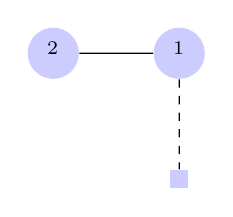
\begin{tikzpicture}
      [scale=.8,auto=left,every node/.style={circle,fill=blue!20}]
      \node (n1) at (3,3) {$\tehole^{1}$};
      \node (n2) at (1,3)  {$\tehole^{2}$};
      \node[rectangle] (i) at (3,1)  {$\tnum$};
    
      \foreach \from/\to in {n1/n2}
        \draw (\from) -- (\to);
       \foreach \from/\to in {n1/i}
        \draw[dashed] (\from) -- (\to);
    
    \end{tikzpicture}
  \caption{Graph of $C_{ex1} = \{ \tehole^{1} \approx \tnum, ~ \tehole^{1} \approx~ \tehole^{2}\}$}
  \label{fig:sub1}
\end{subfigure}
\begin{subfigure}{.39\textwidth}
  \centering
  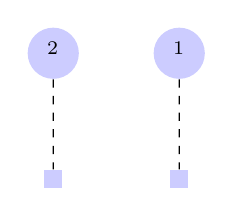
\begin{tikzpicture}
  [scale=.8,auto=left,every node/.style={circle,fill=blue!20}]
  \node (n1) at (3,3) {$\tehole^{1}$};
  \node (n2) at (1,3)  {$\tehole^{2}$};
  \node[rectangle] (i1) at (3,1)  {$\tnum$};
  \node[rectangle] (i2) at (1,1)  {$\tnum$};

   \foreach \from/\to in {n1/i1, n2/i2}
    \draw[dashed] (\from) -- (\to);

\end{tikzpicture}
  \caption{Graph of $C_{ex2} = \{ \tehole^{1} \approx \tnum, ~ \tnum \approx~ \tehole^{2}\}$}
  \label{fig:sub2}
\end{subfigure}
\caption{Sample constraint graphs of primitives}
\label{fig:test}
\end{figure}

In order to extend this logic to binary types like $\tarr{\tau_1}{\tau_2}$, we add nodes and edges for all binary types containing holes. When adding such nodes, we must recursively assess the left and right hand sides of the binary type to see if they contain holes. Any child that containing a hole should also be added as a node. Additionally, if two binary types are constrained to each other, their corresponding left and right hand sides should also be constrained to each other.

As an example of this, consider the constraint set $C_{ex3} = \{ \tarr{\tehole^{1}}{\tehole^{2}} \approx \tarr{\tehole^{3}}{\tnum}  \}$.
Given both types in the constraint contain a hole, they must be added to our graph and connected. Since both are binary arrows, we must constrain their left and right hand sides to each other. This yields the new constraints $\tehole^{1} \approx~ \tehole^{3}$ and $\tehole^{2} \approx~ \tnum$ which must also be reflected in our graph. For $\tehole^{1} \approx~ ?3$, we add two new nodes for each hole and connect them to each other. For $\tehole^{2} \approx~ \tnum$, we only need to create a node for $\tehole^{2}$ and tag it with $\tnum$. An example graph of these associations is provided in figure 8.

\begin{figure}[htbp]
\centering
\begin{tikzpicture}[remember picture,
  inner/.style={circle,draw=blue!50,fill=blue!20,thick,inner sep=3pt},
  innerrect/.style={rectangle,draw=blue!50,fill=blue!20,thick,inner sep=3pt},
  outer/.style={draw=green,fill=green!20,thick,inner sep=10pt}
  ]
  \node[outer,draw=green] (A) {
    \shortstack{
        $Arrow$\\
        \begin{tikzpicture}
          \node [inner] (n1)  {$\tehole^{1}$};
          \node [inner,right=of n1] (n2) {$\tehole^{2}$};
          % \draw[red,thick,->] (n1) -- (n2);
        \end{tikzpicture}
    }
  };
  \node[outer,draw=green,below=of A] (B) {
    \shortstack{
        $Arrow$\\
        \begin{tikzpicture}
          \node [inner] (n3)  {$\tehole^{3}$};
          \node [innerrect,right=of n3] (i) {$\tnum$};
          % \draw[red,thick,->] (n3) -- (i);
        \end{tikzpicture}
    }
  };
  \draw (n1) -- (n3);
  \draw[dashed] (n2) -- (i);
   \draw[thick] (A) -- (B);
\end{tikzpicture}
\caption{Expanded constraint graph of $C_{ex3}$}
\label{fig:test}
\end{figure}

We provide operations detailing the creation of constraint graphs using the metafunctions and types defined earlier in figure 10. We define \textit{link} as a function that retrieves the \textit{PossibleTypeSet}s associated with two \textit{HTyp}s in the map \textit{graph}, computes their union via the \textit{PossibleTypeSet} extension metafunction, and returns an updated graph where the bindings of both \textit{HTyp}s have been updated with the union of their \textit{PossibleTypeSet}s. We define \textit{tag} as a function that retrieves the \textit{PossibleTypeSet} associated with a single \textit{HTyp} \textit{h}, extends it with some primitive \textit{t}, and updates the \textit{HTyp}'s binding with the new extended \textit{PossibleTypeSet}.

\begin{figure}[htbp]
\begin{lstlisting}[escapeinside={(*}{*)}]
let link (graph, t1, t2) =
    let s1 = graph.get(t1) in
    let s2 = graph.get(t2) in
    let s3 = s1 (*$\amalg$*) s2 in
    let graph = graph.insert(t1, s3)in
    let graph = graph.insert(t2, s3) in
    graph;

let tag (graph, t1, t2) =
    let s = graph.get(t1) in
    let s' = s (*$\amalg$*) single(t2) in
    let graph = graph.insert(t1, s') in 
    graph;

let rec construct_graph (graph, constraints) =
    match constraints with
    | [] -> graph
    | hd::tl -> (
        match hd with
        | ((*$\tarr{t1_L}{t1_R}$*), (*$\tarr{t2_L}{t2_R}$*)) ->
            construct_graph(
                graph, 
                (((*$t1_L$*), (*$t2_L$*)))::(((*$t1_R$*), (*$t2_R$*)))::tl
            )
        | ((*$\tehole^{p}$*) as hole, t)
        | (t, (*$\tehole^{p}$*) as hole) ->
            let graph = graph.add(hole, single(hole)) in
            if (contains_hole(t)) then (
                let graph = graph.add(t, single(t)) in
                let graph = link(graph, t, hole) in
                construct_graph(graph, tl)
            ) else (
                let graph = tag(graph, hole, t) in
                construct_graph(graph, tl)
            )
        | _ -> construct_graph(graph, tl)
    )
}

\end{lstlisting}
\vspace{-4px}
 \hrule
\caption{Constraint graph creation algorithm of type hole inference}
\label{fig:algcode}
\end{figure}

With this abstraction in mind, we find that we can determine the \textit{PossibleTypeSet} of any unknown type $\tehole^{p}$ by either conducting a depth first search of each node in the resulting graph, or using union-find to generate connected components as we link nodes during graph construction. We choose to take the latter approach, as it is a much more natural extension of the graph construction algorithm.

% algorithm
When a constraint of the form $A \approx B$ is processed, both A and B's \textit{PossibleTypeSet}s are recovered from the graph and then \textit{link}ed. When computing connected components, the link operation may be adjusted to identify a single representative among $A$ and $B$ via union-find. This representative can then be updated with the union of $A$ and $B$'s \textit{PossibleTypeSet}s. As other \textit{link} operations are performed on $A$ or $B$, union-find allows us to update a single \textit{PossibleTypeSet} shared among all members of their known \textit{connected component}. In this manner, the \texit{PossibleTypeSet} associated with any representative can act as an accumulated connected component across the entirety of \textit{construct\_graph}.

The changes necessary to \textit{link} and \textit{tag} are shown below in figure 11. In order to accommodate this change while ensuring that \textit{PossibleTypeSet}s represented within $Arrow$ \textit{PossibleType}s are also union-found properly, minor adjustments must be made to the type definitions and extension logic discussed above. These are left to Appendix A, where we assume the use of a standard mutable union find library.

% If the operand $T$ of a constraint is num, bool, or arrow, its \textit{PossibleTypeSet} would be single($T$). If it's a type hole $\tehole^{p}$, its \textit{PossibleTypeSet} can be found using the Find operation of the union-find algorithm, which finds the representative \textit{PossibleTypeSet} of which $T$ is a member of.

\begin{figure}[htbp]
\begin{lstlisting}[escapeinside={(*}{*)}]
let link (graph, t1, t2) =
    let rep1 = UnionFind.find(t1) in
    let rep2 = UnionFind.find(t2) in
    let s1 = graph.find(rep1) in
    let s2 = graph.find(rep2) in 
    let merged_rep = UnionFind.union(rep1, rep2) in
    let s' = s1 (*$\amalg$*)_{UF} s2 in
    let graph = graph.insert(merged_rep, s')in
    graph;

let tag (graph, t1, t2) =
    let rep1 = UnionFind.find(t1) in
    let s = graph.get(rep1) in
    let s' = s (*$\amalg_{UF}$*) UnionFind.elem(single(t2)) in
    let graph = graph.insert(t1, s') in 
    graph;
\end{lstlisting}
\vspace{-4px}
 \hrule
\caption{Constraint solving algorithm of type hole inference. Assumes the use of union-findable \textit{PossibleTypeSet}s and $\amalg_{UF}$}
\label{fig:algcode}
\end{figure}

% let link (uf_reps, graph, t1, t2) =
%     let (uf_reps, rep1) = uf_reps.find(uf_reps, t1) in
%     let (uf_reps, rep2) = uf_reps.find(uf_reps, t2) in
%     let s1 = graph.find(rep1) in
%     let s2 = graph.find(rep2) in 
%     let (uf_reps, merged_rep) = uf_reps.union(uf_reps, rep1, rep2) in
%     let s' = s1 (*$\amalg$*)_{UF} s2 in
%     let graph = graph.insert(merged_rep, s')in
%     (uf_reps, graph);

% let tag (uf_reps, graph, t1, t2) =
%     let (uf_reps, rep) = uf_reps.find(uf_reps, t1) in
%     let s = graph.get(t1) in
%     let s' = s (*$\amalg$*) single(t2) in
%     let graph = graph.insert(t1, s') in 
%     (uf_reps, graph);

% let rec construct_graph (uf_reps, graph, constraints) =
%     match constraints with
%     | [] -> graph
%     | hd::tl -> (
%         match hd with
%         | ((*$\tarr{t1_L}{t1_R}$*), (*$\tarr{t2_L}{t2_R}$*)) ->
%             construct_graph(
%                 uf_reps,
%                 graph, 
%                 (((*$t1_L$*), (*$t2_L$*)))::(((*$t1_R$*), (*$t2_R$*)))::tl
%             )
%         | ((*$\tehole^{p}$*) as hole, t)
%         | (t, (*$\tehole^{p}$*) as hole) ->
%             let graph = graph.add(hole, single(hole)) in
%             if (contains_hole(t)) then (
%                 let graph = graph.add(t, single(t)) in
%                 let (uf_reps, graph) = link(uf_reps, graph, t, hole) in
%                 construct_graph(uf_reps, graph, tl)
%             ) else (
%                 let (uf_reps, graph) = tag(uf_reps, graph, hole, t) in
%                 construct_graph(uf_reps, graph, tl)
%             )
%         | _ -> construct_graph(uf_reps, graph, tl)
%     )
% }

% In order to accommodate these changes, some other aspects of \textit{PossibleTypeSet}s and their extension must be changed to ensure representatives are managed properly in union-find. An illustration of these changes is left to Appendix A.

The end result of constraint solving is a mapping from every type hole in the program to a list of suggestions derived from its associated \textit{PossibleTypeSet}. If the user has made no errors when writing their program, each type hole's list of suggestions should contain exactly one type, the type hole's solved type. However, if a program is incomplete or erroneous, the list of suggestions for a type hole may contain multiple types, which have all been constrained to the type hole at some point during constraint collection. The user can then inspect the set of type suggestions and assess which one is correct, and based on the incorrect types suggested, make corrections to the program. In order to ensure failures of the occurs check are caught (for example, $C = \{ \tehole^{1} \approx~ \tarr{\tehole{1}}{\tnum} \}$, we simply assess all nodes during \textit{solve\_constraints} to ensure they don't contain references to themselves in any binary types of their final \textit{PossibleTypeSet}.

\begin{figure}[htbp]
\begin{lstlisting}[escapeinside={(*}{*)}]

let rec fails_occurs (t, s) =
    let arrow_fails (s_L, s_R) =
        single(t) = s_L \vee single(t) = s_R 
            \vee fails_occurs(s_L) \vee fails_occurs(s_R)
    in
    match s with
    | single((*$\tarr{s_L}{s_R}$*)) -> arrow_fails(s_L, s_R)
    | single(_) -> false
    | cons((*$\tarr{s_L}{s_R}$*), tl) -> 
        arrow_fails(s_L, s_R) \vee fails_occurs(tl)
    | cons(_, tl) -> fails_occurs(tl)
    ;

let solve_constraints (constraints) =
    // graph maps from unknown types to their PossibleTypeSet
    let graph = Map.empty() in
    let uf_reps = UnionFind.make(find_all_nodes(constraints)) in
    let (_, graph) = construct_graph(uf_reps, graph, constraints) in
    // suggestions maps from unknown types to their User Suggestions
    let suggestions = Map.empty() in
    let get_final_possible_types = 
        fun key -> (key, graph.get(UnionFind.find(key)), fails_occurs(key, s))
    in
    List.map(get_final_possible_types, graph.keys())
}

\end{lstlisting}
\vspace{-4px}
 \hrule
\caption{Constraint solving algorithm of type hole inference}
\label{fig:algcode}
\end{figure}

Appendix A: OCaml implementation of a union-find compatible \textit{PossibleTypeSet}

\begin{figure}[htbp]
\begin{lstlisting}[escapeinside={(*}{*)}]
open UnionFind

type t = possible_types UnionFind.elem
and possible_type_set = possible_type list
and possible_type =
  | Unknown(provenance)
  | Num
  | Bool
  | Arrow of t * t;

let rec merge_sets_UF (s1: t, s2: t): t =
    let merged_typs = merge_sets (UnionFind.get s1) (UnionFind.get s2) in
    let final_rep = UnionFind.union s1 s2 in
    UnionFind.set final_rep merged_typs;
    final_rep
and merge_sets (s1: possible_type_set, s2: possible_type_set): possible_types = 
    match (s2)
    | [] -> s1
    | s2_hd::s2_hd -> merge_sets (add s1 s2_hd) s2_hd
and add (s: possible_type_set, t: possible_type): possible_type_set =
    match (s)
    | [] -> [t]
    | s_hd::s_tl -> (
        match (s_hd, t)
        | (Arrow(s_hd_L, s_hd_R), Arrow(t_L, t_R)) ->
            let left = merge_sets_UF s_hd_L t_L in
            let right = merge_sets_UF s_hd_R t_R in
            Arrow(left, right)::s_tl
        | _ -> if (s_hd = t) then s else s_hd::(add s_tl t)
    )

let union => if (UnionFind.eq t1 t2) then () else merge_sets_UF t1 t2;
\end{lstlisting}
\vspace{-4px}
 \hrule
\caption{An Implementation of \textit{PossibleTypeSet} using UnionFind}
\label{fig:algcode}
\end{figure}